
%% bare_conf.tex
%% V1.4b
%% 2015/08/26
%% by Michael Shell
%% See:
%% http://www.michaelshell.org/
%% for current contact information.
%%
%% This is a skeleton file demonstrating the use of IEEEtran.cls
%% (requires IEEEtran.cls version 1.8b or later) with an IEEE
%% conference paper.
%%
%% Support sites:
%% http://www.michaelshell.org/tex/ieeetran/
%% http://www.ctan.org/pkg/ieeetran
%% and
%% http://www.ieee.org/

%%*************************************************************************
%% Legal Notice:
%% This code is offered as-is without any warranty either expressed or
%% implied; without even the implied warranty of MERCHANTABILITY or
%% FITNESS FOR A PARTICULAR PURPOSE! 
%% User assumes all risk.
%% In no event shall the IEEE or any contributor to this code be liable for
%% any damages or losses, including, but not limited to, incidental,
%% consequential, or any other damages, resulting from the use or misuse
%% of any information contained here.
%%
%% All comments are the opinions of their respective authors and are not
%% necessarily endorsed by the IEEE.
%%
%% This work is distributed under the LaTeX Project Public License (LPPL)
%% ( http://www.latex-project.org/ ) version 1.3, and may be freely used,
%% distributed and modified. A copy of the LPPL, version 1.3, is included
%% in the base LaTeX documentation of all distributions of LaTeX released
%% 2003/12/01 or later.
%% Retain all contribution notices and credits.
%% ** Modified files should be clearly indicated as such, including  **
%% ** renaming them and changing author support contact information. **
%%*************************************************************************


% *** Authors should verify (and, if needed, correct) their LaTeX system  ***
% *** with the testflow diagnostic prior to trusting their LaTeX platform ***
% *** with production work. The IEEE's font choices and paper sizes can   ***
% *** trigger bugs that do not appear when using other class files.       ***                          ***
% The testflow support page is at:
% http://www.michaelshell.org/tex/testflow/


\documentclass[conference]{IEEEtran}
\IEEEoverridecommandlockouts % Don't forget this command!

% Some Computer Society conferences also require the compsoc mode option,
% but others use the standard conference format.
%
% If IEEEtran.cls has not been installed into the LaTeX system files,
% manually specify the path to it like:
% \documentclass[conference]{../sty/IEEEtran}





% Some very useful LaTeX packages include:
% (uncomment the ones you want to load)


% *** MISC UTILITY PACKAGES ***
%
%\usepackage{ifpdf}
% Heiko Oberdiek's ifpdf.sty is very useful if you need conditional
% compilation based on whether the output is pdf or dvi.
% usage:
% \ifpdf
%   % pdf code
% \else
%   % dvi code
% \fi
% The latest version of ifpdf.sty can be obtained from:
% http://www.ctan.org/pkg/ifpdf
% Also, note that IEEEtran.cls V1.7 and later provides a builtin
% \ifCLASSINFOpdf conditional that works the same way.
% When switching from latex to pdflatex and vice-versa, the compiler may
% have to be run twice to clear warning/error messages.







% *** GRAPHICS RELATED PACKAGES ***
%
\ifCLASSINFOpdf
  % \usepackage[pdftex]{graphicx}
  % declare the path(s) where your graphic files are
  % \graphicspath{{../pdf/}{../jpeg/}}
  % and their extensions so you won't have to specify these with
  % every instance of \includegraphics
  % \DeclareGraphicsExtensions{.pdf,.jpeg,.png}
\else
  % or other class option (dvipsone, dvipdf, if not using dvips). graphicx
  % will default to the driver specified in the system graphics.cfg if no
  % driver is specified.
  % \usepackage[dvips]{graphicx}
  % declare the path(s) where your graphic files are
  % \graphicspath{{../eps/}}
  % and their extensions so you won't have to specify these with
  % every instance of \includegraphics
  % \DeclareGraphicsExtensions{.eps}
\fi
% graphicx was written by David Carlisle and Sebastian Rahtz. It is
% required if you want graphics, photos, etc. graphicx.sty is already
% installed on most LaTeX systems. The latest version and documentation
% can be obtained at: 
% http://www.ctan.org/pkg/graphicx
% Another good source of documentation is "Using Imported Graphics in
% LaTeX2e" by Keith Reckdahl which can be found at:
% http://www.ctan.org/pkg/epslatex
%
% latex, and pdflatex in dvi mode, support graphics in encapsulated
% postscript (.eps) format. pdflatex in pdf mode supports graphics
% in .pdf, .jpeg, .png and .mps (metapost) formats. Users should ensure
% that all non-photo figures use a vector format (.eps, .pdf, .mps) and
% not a bitmapped formats (.jpeg, .png). The IEEE frowns on bitmapped formats
% which can result in "jaggedy"/blurry rendering of lines and letters as
% well as large increases in file sizes.
%
% You can find documentation about the pdfTeX application at:
% http://www.tug.org/applications/pdftex





% *** MATH PACKAGES ***
%
%\usepackage{amsmath}
% A popular package from the American Mathematical Society that provides
% many useful and powerful commands for dealing with mathematics.
%
% Note that the amsmath package sets \interdisplaylinepenalty to 10000
% thus preventing page breaks from occurring within multiline equations. Use:
%\interdisplaylinepenalty=2500
% after loading amsmath to restore such page breaks as IEEEtran.cls normally
% does. amsmath.sty is already installed on most LaTeX systems. The latest
% version and documentation can be obtained at:
% http://www.ctan.org/pkg/amsmath





% *** SPECIALIZED LIST PACKAGES ***
%
%\usepackage{algorithmic}
% algorithmic.sty was written by Peter Williams and Rogerio Brito.
% This package provides an algorithmic environment fo describing algorithms.
% You can use the algorithmic environment in-text or within a figure
% environment to provide for a floating algorithm. Do NOT use the algorithm
% floating environment provided by algorithm.sty (by the same authors) or
% algorithm2e.sty (by Christophe Fiorio) as the IEEE does not use dedicated
% algorithm float types and packages that provide these will not provide
% correct IEEE style captions. The latest version and documentation of
% algorithmic.sty can be obtained at:
% http://www.ctan.org/pkg/algorithms
% Also of interest may be the (relatively newer and more customizable)
% algorithmicx.sty package by Szasz Janos:
% http://www.ctan.org/pkg/algorithmicx




% *** ALIGNMENT PACKAGES ***
%
%\usepackage{array}
% Frank Mittelbach's and David Carlisle's array.sty patches and improves
% the standard LaTeX2e array and tabular environments to provide better
% appearance and additional user controls. As the default LaTeX2e table
% generation code is lacking to the point of almost being broken with
% respect to the quality of the end results, all users are strongly
% advised to use an enhanced (at the very least that provided by array.sty)
% set of table tools. array.sty is already installed on most systems. The
% latest version and documentation can be obtained at:
% http://www.ctan.org/pkg/array


% IEEEtran contains the IEEEeqnarray family of commands that can be used to
% generate multiline equations as well as matrices, tables, etc., of high
% quality.




% *** SUBFIGURE PACKAGES ***
%\ifCLASSOPTIONcompsoc
%  \usepackage[caption=false,font=normalsize,labelfont=sf,textfont=sf]{subfig}
%\else
%  \usepackage[caption=false,font=footnotesize]{subfig}
%\fi
% subfig.sty, written by Steven Douglas Cochran, is the modern replacement
% for subfigure.sty, the latter of which is no longer maintained and is
% incompatible with some LaTeX packages including fixltx2e. However,
% subfig.sty requires and automatically loads Axel Sommerfeldt's caption.sty
% which will override IEEEtran.cls' handling of captions and this will result
% in non-IEEE style figure/table captions. To prevent this problem, be sure
% and invoke subfig.sty's "caption=false" package option (available since
% subfig.sty version 1.3, 2005/06/28) as this is will preserve IEEEtran.cls
% handling of captions.
% Note that the Computer Society format requires a larger sans serif font
% than the serif footnote size font used in traditional IEEE formatting
% and thus the need to invoke different subfig.sty package options depending
% on whether compsoc mode has been enabled.
%
% The latest version and documentation of subfig.sty can be obtained at:
% http://www.ctan.org/pkg/subfig




% *** FLOAT PACKAGES ***
%
%\usepackage{fixltx2e}
% fixltx2e, the successor to the earlier fix2col.sty, was written by
% Frank Mittelbach and David Carlisle. This package corrects a few problems
% in the LaTeX2e kernel, the most notable of which is that in current
% LaTeX2e releases, the ordering of single and double column floats is not
% guaranteed to be preserved. Thus, an unpatched LaTeX2e can allow a
% single column figure to be placed prior to an earlier double column
% figure.
% Be aware that LaTeX2e kernels dated 2015 and later have fixltx2e.sty's
% corrections already built into the system in which case a warning will
% be issued if an attempt is made to load fixltx2e.sty as it is no longer
% needed.
% The latest version and documentation can be found at:
% http://www.ctan.org/pkg/fixltx2e


%\usepackage{stfloats}
% stfloats.sty was written by Sigitas Tolusis. This package gives LaTeX2e
% the ability to do double column floats at the bottom of the page as well
% as the top. (e.g., "\begin{figure*}[!b]" is not normally possible in
% LaTeX2e). It also provides a command:
%\fnbelowfloat
% to enable the placement of footnotes below bottom floats (the standard
% LaTeX2e kernel puts them above bottom floats). This is an invasive package
% which rewrites many portions of the LaTeX2e float routines. It may not work
% with other packages that modify the LaTeX2e float routines. The latest
% version and documentation can be obtained at:
% http://www.ctan.org/pkg/stfloats
% Do not use the stfloats baselinefloat ability as the IEEE does not allow
% \baselineskip to stretch. Authors submitting work to the IEEE should note
% that the IEEE rarely uses double column equations and that authors should try
% to avoid such use. Do not be tempted to use the cuted.sty or midfloat.sty
% packages (also by Sigitas Tolusis) as the IEEE does not format its papers in
% such ways.
% Do not attempt to use stfloats with fixltx2e as they are incompatible.
% Instead, use Morten Hogholm'a dblfloatfix which combines the features
% of both fixltx2e and stfloats:
%
% \usepackage{dblfloatfix}
% The latest version can be found at:
% http://www.ctan.org/pkg/dblfloatfix




% *** PDF, URL AND HYPERLINK PACKAGES ***
%
%\usepackage{url}
% url.sty was written by Donald Arseneau. It provides better support for
% handling and breaking URLs. url.sty is already installed on most LaTeX
% systems. The latest version and documentation can be obtained at:
% http://www.ctan.org/pkg/url
% Basically, \url{my_url_here}.




% *** Do not adjust lengths that control margins, column widths, etc. ***
% *** Do not use packages that alter fonts (such as pslatex).         ***
% There should be no need to do such things with IEEEtran.cls V1.6 and later.
% (Unless specifically asked to do so by the journal or conference you plan
% to submit to, of course. )


% correct bad hyphenation here
\hyphenation{op-tical net-works semi-conduc-tor}
\usepackage{hyperref}
\usepackage{comment}
\usepackage{graphicx}

% correct bad hyphenation here
\hyphenation{op-tical net-works semi-conduc-tor}

\renewcommand{\vec}[1]{\mathbf{#1}}
\usepackage{amssymb}

%\usepackage{algorithm}
%\usepackage{algorithmic}
\usepackage{url}
\graphicspath{{"D:/PhDWorkwc/PhDWorks/trunk/trunk/CACO/diagrams/"}{"C:/PhDWorks/CACO/diagrams/"}}
%C:/Users/Yang Shi/Dropbox/PhDWorks/trunk/CACO/diagrams/D:/Dropbox/PhDWorks/trunk/CACO/diagrams/

\usepackage[utf8]{inputenc}

\usepackage{listings,lstautogobble}
\usepackage{color}

\definecolor{codegreen}{rgb}{0,0.6,0}
\definecolor{codegray}{rgb}{0.5,0.5,0.5}
\definecolor{codepurple}{rgb}{0.58,0,0.82}
\definecolor{backcolour}{rgb}{0.95,0.95,0.92}

\lstdefinestyle{mystyle}{
	backgroundcolor=\color{backcolour},   
	commentstyle=\color{codegreen},
	keywordstyle=\color{magenta},
	numberstyle=\tiny\color{codegray},
	stringstyle=\color{codepurple},
	basicstyle=\footnotesize,
	breakatwhitespace=false,         
	breaklines=true,                 
	captionpos=b,                    
	keepspaces=true,                 
	numbers=left,                    
	numbersep=5pt,                  
	showspaces=false,                
	showstringspaces=false,
	showtabs=false,                  
	tabsize=2,
	autogobble=true
}

\lstset{style=mystyle}
\usepackage[justification=centering]{caption}
\usepackage{algpseudocode}
\usepackage[]{algorithm2e}
\usepackage{amsmath}
\begin{document}
%
% paper title
% Titles are generally capitalized except for words such as a, an, and, as,
% at, but, by, for, in, nor, of, on, or, the, to and up, which are usually
% not capitalized unless they are the first or last word of the title.
% Linebreaks \\ can be used within to get better formatting as desired.
% Do not put math or special symbols in the title.
\title{Bare Demo of IEEEtran.cls\\ for IEEE Conferences}


% author names and affiliations
% use a multiple column layout for up to three different
% affiliations
\author{\IEEEauthorblockN{Yang Shi}
\IEEEauthorblockA{Department of Electrical and\\Computer Engineering\\
Portland State University\
Portland, Oregon 97201\\
Email: yangshi.psu@gmail.com}
\and
\IEEEauthorblockN{Homer Simpson}
\IEEEauthorblockA{Twentieth Century Fox\\
Springfield, USA\\
Email: homer@thesimpsons.com}
\and
\IEEEauthorblockN{Peter Griffin}
\IEEEauthorblockA{Starfleet Academy\\
San Francisco, California 96678--2391\\
Telephone: (800) 555--1212\\
Fax: (888) 555--1212}}

% conference papers do not typically use \thanks and this command
% is locked out in conference mode. If really needed, such as for
% the acknowledgment of grants, issue a \IEEEoverridecommandlockouts
% after \documentclass

% for over three affiliations, or if they all won't fit within the width
% of the page, use this alternative format:
% 
%\author{\IEEEauthorblockN{Michael Shell\IEEEauthorrefmark{1},
%Homer Simpson\IEEEauthorrefmark{2},
%James Kirk\IEEEauthorrefmark{3}, 
%Montgomery Scott\IEEEauthorrefmark{3} and
%Eldon Tyrell\IEEEauthorrefmark{4}}
%\IEEEauthorblockA{\IEEEauthorrefmark{1}School of Electrical and Computer Engineering\\
%Georgia Institute of Technology,
%Atlanta, Georgia 30332--0250\\ Email: see http://www.michaelshell.org/contact.html}
%\IEEEauthorblockA{\IEEEauthorrefmark{2}Twentieth Century Fox, Springfield, USA\\
%Email: homer@thesimpsons.com}
%\IEEEauthorblockA{\IEEEauthorrefmark{3}Starfleet Academy, San Francisco, California 96678-2391\\
%Telephone: (800) 555--1212, Fax: (888) 555--1212}
%\IEEEauthorblockA{\IEEEauthorrefmark{4}Tyrell Inc., 123 Replicant Street, Los Angeles, California 90210--4321}}




% use for special paper notices
%\IEEEspecialpapernotice{(Invited Paper)}




% make the title area
\maketitle

% As a general rule, do not put math, special symbols or citations
% in the abstract
\begin{abstract}
The abstract goes here.
\end{abstract}

% no keywords

% Determinisitic
% Statistical
% Coverage Rate


% For peer review papers, you can put extra information on the cover
% page as needed:
% \ifCLASSOPTIONpeerreview
% \begin{center} \bfseries EDICS Category: 3-BBND \end{center}
% \fi
%
% For peerreview papers, this IEEEtran command inserts a page break and
% creates the second title. It will be ignored for other modes.
\IEEEpeerreviewmaketitle

% *** CITATION PACKAGES ***
%
%\usepackage{cite}
% cite.sty was written by Donald Arseneau
% V1.6 and later of IEEEtran pre-defines the format of the cite.sty package
% \cite{} output to follow that of the IEEE. Loading the cite package will
% result in citation numbers being automatically sorted and properly
% "compressed/ranged". e.g., [1], [9], [2], [7], [5], [6] without using
% cite.sty will become [1], [2], [5]--[7], [9] using cite.sty. cite.sty's
% \cite will automatically add leading space, if needed. Use cite.sty's
% noadjust option (cite.sty V3.8 and later) if you want to turn this off
% such as if a citation ever needs to be enclosed in parenthesis.
% cite.sty is already installed on most LaTeX systems. Be sure and use
% version 5.0 (2009-03-20) and later if using hyperref.sty.
% The latest version can be obtained at:
% http://www.ctan.org/pkg/cite
% The documentation is contained in the cite.sty file itself.

\section{Introduction}
% no \IEEEPARstart
Software testing takes fifty percent of time in the overall software development cycle time. It is vital to have an efficient and high quality test data generation mechanism. Software automated testing aims at generating high quality test cases without human efforts. It is an active research area since thirty years ago and it is paid more attention recently. Coverage-driven software testing often refers to structural testing in which testing requirements are specified in terms of cover elements. A type of cover elements related to structure of SUT(System Under Test) is usually defined by to statement, branch or path of program. Another type of cover elements related to specification of SUT is usually defined by properties or functions. They are generally described in the form of formal language. \\

Coverage driven structural testing follows two principles: deterministic and statistical. In deterministic testing scheme, the quality of test set is measured directly by counting the number of cover elements being triggered. Higher quality indicates more cover elements being exercised. The quality of the test set is built up by evaluating the quality of each input vector. Automated Deterministic Structural Testing automate the process of constructing input vector set. A typical work includes the branch distance measure, approximation level etc*. \\  

In statistical testing scheme, the quality of test set refers to the probability that this set could exercising each cover element at least once. In general, the test set is sampled from a probability distribution(or input profile) over the input domain space. An input distribution exhibiting a higher probability of exercising each cover element results in a higher quality of statistical test set.\\

Constructing such input profile can be accomplished by analyzing the program's control flow. One needs to identify each path of the program and its corresponding subset of input vectors. Then, proper probability is assigned to it. Apparently, It is infeasible work for non-toy program. \\

Automated Statistical Structural Testing(ASST) automate the process of constructing input profile.[Clark \& Simon] use a search-based method to derive the optimal distribution. They demonstrate that the automated search is able to derive near-optimal distribution. The main problem is search efficiency: On one hand, Curse of uncertainty caused by fitness estimation could significantly decrease the convergence speed. On the other hand, a cover element corresponds to a small size of sub-domain or many non-consecutive sub-domains result in the search hard to detect the high fitness region.\\

To minimize the negative effects on search efficiency, We improve the original design from following aspects: 
\begin{itemize}
	\item Input distribution model: we use sum of weighted Gaussian distributions
	\item Search algorithm: we adopt cell based genetic algorithm approach.\\	
\end{itemize}

The rest of this paper is organized as follows. Section II presents related work of statistical testing. Section III gives background knowledge and notations. Section IV gives brief review of cell based genetic algorithm. Section V represents the implementation of using cell base GA to search for near-optimal input profile. Section VI shows experiments and results. Section VII is the conclusion.\\

\section{Problem Modeling}
Suppose a black box system produces labels for a seeded input vector, and the input vector has a pre-defined domain range. Further, a probability distribution is constructed to generate input vectors for the system. The aim is to construct a probability distribution over the input domain space to satisfy some constraint. One of the them is described in the following: for each label can be produced by the system, the probability distribution guarantees that each label has equal probability being triggered.

Due to the reason that there is no information available to the system, the only method to gain the information is to draw samples from a probability distribution and then run the black box system against these samples to acquire the partial knowledge. With the learned knowledge, one can create or improve the probability distribution. This "trail and error" process is iterated a mount of times until the optimal/near optimal probability distribution is found.

Let's suppose the input of the system is denoted as \(x\). The set of labels output by the system is denoted as \(C = \{c_1,c_2 ... c_i\}\). Let \(S_{c_{i}}\) denotes the set of input vectors labeled as \(c_{i}\). Furthermore, lets suppose \(\bigcap_{j=1}^i S_{c_{j}} = \emptyset\). 

Let \(P(x)\) be the discrete input distribution. The probability of a test input produced by \(P(x)\) that triggers \(c_{i}\) is defined in the following:\[\label{eq:ability}p_{c_i} = \sum_{x \in S_{c_i}} P(x)\]

Namely, \(p_{c_{i}}\) is the probability of triggering any one of input vectors inside of \(S_{c_i}\).
In other words, \(p_{c_{i}}\) represents the level of confidence  of an input distribution to trigger the cover element \(c_{i}\) by a sampled input vector.

From above equation, Calculating \(p_{c_{i}}\) requires to know each element in the \(S_{c_{i}}\) which can only be obtained by exhaustively running the system over the entire input domain space. Therefore it is necessary to estimate the probability.
Suppose a test set which consists of \(n\) input vectors are labeled after run the system. Two outcomes are taken into consideration: sampled test input triggers \(c_{i}\) or it does not trigger \(c_{i}\). Let \(p_{*}\) denotes the actual probability of triggering \(c_{i}\). We can derive that the number of input vectors labeled \(c_{i}\) in the test set follows a binomial distribution defined as follows:
\[P(n_{c_{i}}) = \binom{n}{n_{c_{i}}}p_{*}^{n_{c_{i}}}\cdot (1-p_{*})^{(n-n_{c_{i}})} \]

In the view of frequentist statistics, the probability can be estimated by using the maximum likelihood estimation method(MLE) \cite{mle}, and the unbiased estimator of binomial distribution is in the following:
\[ \label{eq:estp}
\tag{5}
\hat{p_{c_i}} = \frac{n_{c_i}}{n}\]

Therefore, the estimated probability of triggering label \(c_i\) by the input distribution can be estimated by the fraction of the number of input vectors triggered \(c_i\) in the test set and the size of the test set.
\subsection{Probability Distribution Modeling}
The input domain space is a set of input vectors. The construction of probability distribution can be viewed as the process of assign weights to each input vector. Then the probability of sampling a input vector is simply the fraction of weight assigned to the weight and the total weights.
Then the optimization problem is to find a suitable set of weights for each input vector. Then the dimension of the optimization problem is equal to the size of input domain space, which is huge and impossible to optimize. Therefore, we divide the input domain space into several equivalent sub-domains, and the weights are only assigned to the sub-domain space rather than each input vector. If a sub-domain is selected, a input vector in the sub-domain is uniformly sampled.
\subsubsection{Split the input domain space} The domain range of each variable is divided into several equivalent sub-domains, and the sub-domain range of variable \(x_{i}\) is denoted as \(\Delta x_{i}\). Then the elements with in the range defined in below form a sub-domain. 
\[
 \begin{bmatrix}
k_{1} \\
: \\
k_{d}
\end{bmatrix}^T
 \begin{bmatrix}
 \Delta_{1} \\
: \\
\Delta_{d}
\end{bmatrix}
\leq
 \begin{bmatrix}
	x_{1} \\
    : \\
x_{d}
\end{bmatrix}
<
 \begin{bmatrix}
x_{1} + \Delta_{1} \\
: \\
x_{d} + \Delta_{d}
\end{bmatrix}
\]
where \(k_{1}\) represents the index of the sub-domain of variable \(x_{i}\). Therefore the low bound of the sub-domain of \(x_{i}\) is \(k_{i}*\Delta_{i}\). The high bound is the vector addition of \(x\) and \(\Delta\).

\subsubsection{Probability Distribution Model}
To accommodate the sub-domain based probability distribution, the model is chosen to be the \emph{mixture of Multi-variable uniform distributions} (MUD).
The generalized mixture of uniform distributions has the following form:
\[U(\vec{x},\theta_{1},\theta_{2},...,\theta_{n}) = \sum_{i = 1}^{j}\phi_{i}u_{i}(x,\theta_{i*2-1},\theta_{i*2})\]

\begin{figure}[t]
	\hspace*{0.2cm}
	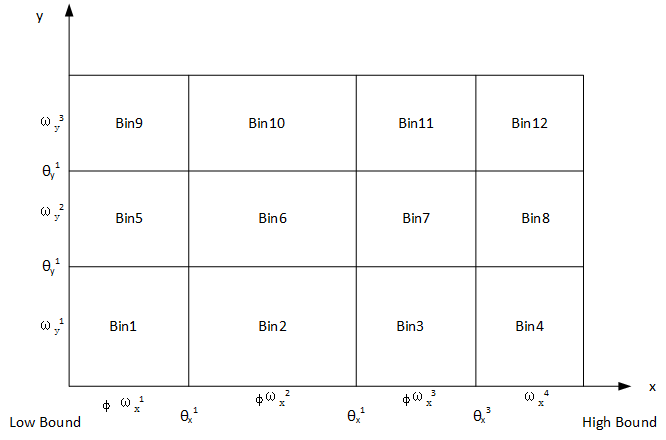
\includegraphics[scale=0.5]{Bin.png}
	\caption{Top view of input domain split into sub-domains for two variables}
	\label{fig:bins}
\end{figure}
where \(\phi_{i}\) refers to the weight of i'th component, and the total weight is summed up to \(1\).

\(u_{i}(\vec{x},\theta_{i*2-1},\theta_{i*2})\) represents the i-th component of \(MUD\). It is a multi-dimensional uniform distribution with low bound denoted as \(\theta_{i*2-1}\) and up bound denoted as \(\theta_{i*2}\).\\


Mapping from the sub-domain to \(MUD\), each uniform component corresponds to a sub-domain space where each input vector in the sub-domain is sampled uniformly; The low bound and high bound are matched into the low end and high end of the uniform distribution. The weight \(\phi_{i}\) of i-th component in \(MUD\) is calculated by the equation in below.
\begin{equation}
\phi_{i} = \frac{\prod_{d=1}^{dim}\omega_{d}^i}{\sum_{i = 1}^{j} \prod_{d=1}^{dim}\omega_{d}^i}
\end{equation}
where \(dim\) represents the dimension of the input domain space. \(\phi_{i}\) represents the total weight of the i-th \(bin\). The total weight is the product of weights in each dimension. Each \(\phi_{i}\) is normalized so that all of the weights in \(MUD\) is summed up to 1.

\subsection{The Memetic MOGA}
The goal of the problem is to optimize the weights \(\omega\) for each sub-domain. From the empirical study
\subsection{Fitness Estimation}
\subsection{Local Search}
\subsection{A Case Study}

\section{Application: Statistical Structural Testing}
We start from essential definitions\\\\
\noindent\emph{Definition 1}: A Branch Cover Element \(c_i\) is an indication of a branch being taken or not taken by running SUT with a given input vector.\\\\
\noindent\emph{Definition 2}: An Instrumented SUT is the SUT with inserted lines of code into each branch which output branch cover elements being triggered by running SUT against a set of input vectors. Formally, An SUT has \(n\) inputs, denoted as \(\vec{v}=(v_1,v_2...v_n)\). Each input has a domain \(d_{v_i}\) = \([L_{d_{v_i}},U_{d_{v_i}}]\). The input domain space \(D\) has \(k = |d_{v_1}|*|d_{v_2}|*...*|d_{v_n}|\) input vectors. An SUT which contains \(n\) branches has \(2*n\) branch cover elements denoted as \(C = {\{c_1,c_2 ...c_n, c_{2n}\}}\). An Instrumented SUT takes an input vector \(\vec{x_i}\), output a set of cover elements \(c_{x_i} = \{c_{x_i}| \forall c \in C, x_i\ triggers\ c\}\)  \\\\
In this article, We only consider the SUTs which inputs are independent from each other.\\\\

\noindent\emph{Definition 3}: An input profile denoted as \(f(x) \) is a probability distribution of selecting input vectors \(x_i\) over input domain space.The probability of triggering a cover element \(c_i\) by sampling from \(f(x)\) is as follow:\[P_{c_i} = \sum_{x \in s} f(x), s \subseteq D \ and \ x \in s \ triggers {c_i}\]. 

\noindent\emph{Definition 4}: Quality of statistical input vector set is a measurement of goodness of a test set with respect to branch cover elements. We denote size of input vector set \(n\). The quality \(q_{c_i}\) with respect to cover element \(c_i\)  is defined as follow: \[q_{c_i} = 1-(1-P_{c_i})^n\]
   \ \ Usually, we set \(q = q_{c_1} = q_{c_2} = ... = q_{c_n}\).To improve the quality of statistical input vector set, one can either increase the size of test set or can find an input profile that has a higher \(p_{c_i}\) value. However, a high efficient input vector set requires less number of input vectors to achieve an equivalent level of quality with respect to all of cover elements. Search based statistical testing aims at searching for a well-suited input profile which satisfies the user's requirement on efficiency in terms of \(\tau_{c_i}\). Statistical test data generation requires following steps:
 \begin{enumerate}
 	\item \textbf{Searching for a well-suited input distribution}: Normally, we preset the target value of \(p_{c_i}\) as \(\tau_{c_i}\). A search algorithm is conducted to find a qualified \(f(x)\) s.t \(\forall c_i \in C, p_{c_i} >= \tau_{c_i}\).
 	\item \textbf{Determining the size of test vector set}: With given \(p_{c_i}\) from last step, the size of input vectors \(n\) can be derived from following equation \[n = \frac{log(1-q)}{log(1-p_{c_i})},\quad where \ p_{c_i} = \min\{p_{c_k}, c_k \in C\}\]   
 \end{enumerate}
 
 There exists a notable problem on the evaluation of \(p_{c_i}\). The exact \(p_{c_i}\) calculation requires to exhaustively run SUT over the entire input domain \(D\) in order to retrieve the maximum subset of \(D\) covers \(c_i\). It is most of time unrealistic even for a small program. Instead of exact calculation, we could estimate \(p_{c_i}\) from samples. Suppose \(n\) samples are drawn from \(f(x)\). after running SUT against the sample set, there are \ \(n_{c_i}\) input vectors exercising \(c_i\). The estimation of \(p_{c_i}\) is as follow: \[\hat{p_{c_i}} = \frac{n_{c_i}}{n}\] \ \ To increase the accuracy of estimation, ensemble average method can be adopted. The detail algorithm is described in the later sections.
 
\section{Cell Based Genetic Algorithm}
 Cell based genetic algorithm is proposed by Amer [3]. Their objective is to automatically generate a proper directives for random test generators in order to test circuits that are written by SystemC. The directives are cells over the input domain with assigned weights indicating the importance of a cell in terms of number of functional cover points being covered. The set of input vectors are randomly generated but guided by the directives. In this section, we give a briefly review on general GA, cell based encoding scheme and the Inter-Cell crossover operator.
 \subsection{Cell Based Encoding Scheme}
 \noindent\emph{Definition 5}: A cell represents a sub-input-domain \(d_i\), \(d_i \subseteq D\). A cell consists of a lower bound vector \(\vec{L_i}\), an upper bound vector \(\vec{H_i}\) and a weight parameter \(w_i\).  \\
  
 A genotype is encoded as an array of \(n\) disjoint cells. Each gene represented as a cell contains three attributes: \((\vec{L_i},\vec{H_i},w_i)\). 
 
 
 \subsection{Inter-Cell Crossover}
 Given two chromosomes \(Chrome_i\) and \(Chrome_j\), Inter-Cell Crossover creates new chromosomes by two set operations listed in below:
 \begin{itemize}
 	\item \(Chrome_i \cup Chrome_j\): One chromosome is created by the union operation. The weight of new merged cell is proportional to the weight and size of each cell involved in the union process.
 	\item \(Chrome_i \cap Chrome_j\): The other chromosome is created by the intersection operation. The weight of new intersected cell is the average of weights of the overlapped cells. \\
 \end{itemize}
 
 As with the standard genetic algorithm, cell based GA selects chromosomes for reproduction by roulette wheel selection. Its mutation operators helps evolution process from preventing the premature convergence. Elitism is adopted to ensure the evolution process does not discard the currently best solutions by copying a small potion of the best solutions into the next generation.\\

\section{Searching Input Distribution by CBGA}
Given a population of initial input distributions \(P=\{f_1(x), f_2(x), ... f_n(x)\}\), our goal is to find an optimal input distribution that maximizes \(p_{c_i}\ where\ p_{c_i} = \min\{p_{c_k}, c_k \in C\}\). As mentioned above, GA consists of genotype encoding, genetic operators, and fitness evaluation. In what follows, we discuss the implementation details of each component in solving the input distribution optimization problem.
\subsection{Representation of Input Distribution}

The input distribution \(f(x)\) is represented as a sum of weighted Gaussian distributions. Formally, let \(n\) denotes the number of Gaussian distributions; \(\vec{\mu_i}\), \(\ \vec{\sigma_i}\) and \(a_i\) denotes the mean vector, standard deviation vector and weight of i'th Gaussian distribution. The equation of \(f(x)\) is defined as follow:\[f(x) = \sum_{i=1}^{n}a_iN_i(x,\vec{\mu_i},\sigma_i)\] The total number of parameters for GA to optimize is: \(P = 3*|\vec{\mu_i}|*n + n\).\\

GA can be benefit from using sum of weighted Gaussian distributions in the following reasons:
\begin{enumerate}
	\item It is suited for branch cover elements with discontinuous sub-input domain. Each Gaussian component is represented as a gene in its genotype. As evolution keeps moving forward, a Gaussian component which takes effect on a solitary but high fitness sub-input-domain space could be kept in the natural selection phase.\\
	\item It creates a smooth fitness landscape due to the bell shaped curve of each Gaussian component and the averaging effect of the sum operation. \\ 
\end{enumerate}

Sampling a PDF composed by sum of \(n\) weighted Gaussian distributions can be divided into a two-step process{[2]}.
The first step is to choose a Gaussian component. we use roulette wheel selection method. The probability of choosing the i'th component \(N_i\) is computed by the following equation:\[p_i = \frac{w_i}{\sum_{k=1}^{n}w_k}\] The second step is to sample the selected Gaussian component \(N_i\). This is a standard process which can be accomplished by many piratical methods. For instance, the Box-Muller method{[4]}.
\subsection{Encoding}
As we discussed above, a genotype \(g_i\) which has \(n\) genes are encoded as follow: 
\[G_i=[(\vec{L_1},\vec{H_1},w_1),\ (\vec{L_2},\vec{H_2},w_2)\ ...\ (\vec{L_i},\vec{H_i},w_i),\ (\vec{L_n},\vec{H_n},w_n)]\]
where \(\vec{L_i},\vec{H_i} \in \mathbb{R}^d, w_i \in \mathbb{R+}, d = |\vec{H_i}|\).
Each Gaussian component is mapped into a corresponding cell with same index. The following equations convert the parameters of i'th cell into parameters of i'th Gaussian component:
\begin{enumerate}
	\item \(a_i = w_i\),
	\item \(\vec{\mu_i} = \frac{\vec{L_i}+\vec{H_i}}{2}\),
	\item \(\vec{\sigma_i} = (\vec{H_i} - \vec{\mu_i})\)\\
\end{enumerate}
We require the Gaussian component to be centered at the mean of the cell and samples drawn from the Gaussian should have the probability of \(68.26\%\) hitting the region of the cell. The weight of Gaussian component is equivalent to the weight of the cell.
\subsection{Recombination}
The crossover operator selects two parent solutions randomly from the population and recombines them to form two offspring. We use \emph{Inner-Cell Crossover} as crossover operator.
Specially, Suppose two genotypes \(G_1\) and \(G_2\) performs Inner Cell Crossover. Gene \(g_{12}\) indicated as the gene at position one of \(G_2\) overlaps with \(g_{11}\) and  \(g_{12}\), as shown in figure{ x}. After inner cell crossover, \(New\ G_1\) is created by union operator, \(New\ G_2\) is created by intersect operator. The value of their attributes are listed in table below:
\begin{center}
	\begin{tabular}{ | c | c | c | c | c | c | c |}
		\hline
		 &\(\vec{L}_1\)& \(\vec{H}_1\) & \(w_1\) & \(\vec{L}_2\) & \(\vec{H}_2\) & \(w_2\) \\ \hline
		\(New\ G_1\) & \(\vec{L}_{g_{11}}\) & \(\vec{H}_{g_{21}}\) & \(K\) &  -&  -& -\\ \hline
		\(New\ G_2\) & \(\vec{L}_{g_{12}}\) & \(\vec{H}_{g_{11}}\) & \(\frac{w_{g_{11}} + w_{g_{12}}}{2}\) & \(\vec{L}_{g_{21}}\) & \(\vec{H}_{g_{12}}\) & \(\frac{w_{g_{21}} + w_{g_{12}}}{2}\) \\ \hline
		\hline
	\end{tabular}
\ \\ \ \\ \ \\
\(
K = \frac{(w_{g_{11}}*(\vec{H}_{g_{11}} - \vec{L}_{g_{11}}) + 
	w_{g_{21}}*(\vec{H}_{g_{21}} - \vec{L}_{g_{21}}) + 
	w_{g_{12}}*(\vec{H}_{g_{12}} - \vec{L}_{g_{12}}))}{\vec{H}_{g_{21} - \vec{L}_{g_{11}}}}
\)
\end{center} 

\subsection{Mutation}
The mutation operator mutates a genotype to create a new solution. We adopt the following mutation operators from CBGA, which are:
\begin{itemize}
	\item insert or delete a cell
	\item Shift or adjust a cell
	\item Change cell's weight \\
\end{itemize}
\ \ All of the operations should not violate the disjoint property of each cell. When a genotype is chosen for mutation, one of the above five operators is randomly selected by performing roulette wheel selection method. The weight of each operator is pre-defined by user.
\subsection{Fitness Evaluation}
\section{Experimental Results}
  SUT introduction\\
  how to initialize\\
  what are the parameters\\
  experiment result\\
  Compare table\\




%[2] C. Blum and K. Socha. Training feed-forward neural
%networks with ant colony optimization: An application to
%pattern classification. In 5th International Conference on
%Hybrid Intelligent Systems, pages 233–238, 2005.

%[4] G. Box and M. Muller. A note on the generation of random
%normal deviates. Annals. Math. Stat., 29:610–611, 1958.
  
% An example of a floating figure using the graphicx package.
% Note that \label must occur AFTER (or within) \caption.
% For figures, \caption should occur after the \includegraphics.
% Note that IEEEtran v1.7 and later has special internal code that
% is designed to preserve the operation of \label within \caption
% even when the captionsoff option is in effect. However, because
% of issues like this, it may be the safest practice to put all your
% \label just after \caption rather than within \caption{}.
%
% Reminder: the "draftcls" or "draftclsnofoot", not "draft", class
% option should be used if it is desired that the figures are to be
% displayed while in draft mode.
%
%\begin{figure}[!t]
%\centering
%\includegraphics[width=2.5in]{myfigure}
% where an .eps filename suffix will be assumed under latex, 
% and a .pdf suffix will be assumed for pdflatex; or what has been declared
% via \DeclareGraphicsExtensions.
%\caption{Simulation results for the network.}
%\label{fig_sim}
%\end{figure}

% Note that the IEEE typically puts floats only at the top, even when this
% results in a large percentage of a column being occupied by floats.


% An example of a double column floating figure using two subfigures.
% (The subfig.sty package must be loaded for this to work.)
% The subfigure \label commands are set within each subfloat command,
% and the \label for the overall figure must come after \caption.
% \hfil is used as a separator to get equal spacing.
% Watch out that the combined width of all the subfigures on a 
% line do not exceed the text width or a line break will occur.
%
%\begin{figure*}[!t]
%\centering
%\subfloat[Case I]{\includegraphics[width=2.5in]{box}%
%\label{fig_first_case}}
%\hfil
%\subfloat[Case II]{\includegraphics[width=2.5in]{box}%
%\label{fig_second_case}}
%\caption{Simulation results for the network.}
%\label{fig_sim}
%\end{figure*}
%
% Note that often IEEE papers with subfigures do not employ subfigure
% captions (using the optional argument to \subfloat[]), but instead will
% reference/describe all of them (a), (b), etc., within the main caption.
% Be aware that for subfig.sty to generate the (a), (b), etc., subfigure
% labels, the optional argument to \subfloat must be present. If a
% subcaption is not desired, just leave its contents blank,
% e.g., \subfloat[].


% An example of a floating table. Note that, for IEEE style tables, the
% \caption command should come BEFORE the table and, given that table
% captions serve much like titles, are usually capitalized except for words
% such as a, an, and, as, at, but, by, for, in, nor, of, on, or, the, to
% and up, which are usually not capitalized unless they are the first or
% last word of the caption. Table text will default to \footnotesize as
% the IEEE normally uses this smaller font for tables.
% The \label must come after \caption as always.
%
%\begin{table}[!t]
%% increase table row spacing, adjust to taste
%\renewcommand{\arraystretch}{1.3}
% if using array.sty, it might be a good idea to tweak the value of
% \extrarowheight as needed to properly center the text within the cells
%\caption{An Example of a Table}
%\label{table_example}
%\centering
%% Some packages, such as MDW tools, offer better commands for making tables
%% than the plain LaTeX2e tabular which is used here.
%\begin{tabular}{|c||c|}
%\hline
%One & Two\\
%\hline
%Three & Four\\
%\hline
%\end{tabular}
%\end{table}


% Note that the IEEE does not put floats in the very first column
% - or typically anywhere on the first page for that matter. Also,
% in-text middle ("here") positioning is typically not used, but it
% is allowed and encouraged for Computer Society conferences (but
% not Computer Society journals). Most IEEE journals/conferences use
% top floats exclusively. 
% Note that, LaTeX2e, unlike IEEE journals/conferences, places
% footnotes above bottom floats. This can be corrected via the
% \fnbelowfloat command of the stfloats package.




\section{Conclusion}
The conclusion goes here.




% conference papers do not normally have an appendix


% use section* for acknowledgment
\section*{Acknowledgment}


The authors would like to thank...





% trigger a \newpage just before the given reference
% number - used to balance the columns on the last page
% adjust value as needed - may need to be readjusted if
% the document is modified later
%\IEEEtriggeratref{8}
% The "triggered" command can be changed if desired:
%\IEEEtriggercmd{\enlargethispage{-5in}}

% references section

% can use a bibliography generated by BibTeX as a .bbl file
% BibTeX documentation can be easily obtained at:
% http://mirror.ctan.org/biblio/bibtex/contrib/doc/
% The IEEEtran BibTeX style support page is at:
% http://www.michaelshell.org/tex/ieeetran/bibtex/
%\bibliographystyle{IEEEtran}
% argument is your BibTeX string definitions and bibliography database(s)
%\bibliography{IEEEabrv,../bib/paper}
%
% <OR> manually copy in the resultant .bbl file
% set second argument of \begin to the number of references
% (used to reserve space for the reference number labels box)
\begin{thebibliography}{1}

\bibitem{IEEEhowto:kopka}
H.~Kopka and P.~W. Daly, \emph{A Guide to \LaTeX}, 3rd~ed.\hskip 1em plus
  0.5em minus 0.4em\relax Harlow, England: Addison-Wesley, 1999.

\end{thebibliography}




% that's all folks
\end{document}



%%%%%%%%%%%%%%%%%%%%%%%%%%NOTES%%%%%%%%%%%%%%%%%%%%%%%%%%%%%%%%%

% A function \(g(x)\) assigns the value of weight parameter into each input vector in \(d_i\) is %defined as follow:
%\[
%g(\vec{x},\vec{L_i},\vec{H_i}) = 
%\left\{
%\begin{array}{lr}
%w_i,  &\vec{x} \in [\vec{L_i},\vec{H_i}] \\
%0, &otherwise
%\end{array}
%\right\}
%\]

